\documentclass[a4paper,10pt]{scrartcl}
\usepackage[utf8]{inputenc}

% Title Page
\title{Working with Files and Data, including geospatial methods and plotting}
\author{Andrew D. Wickert}

\usepackage{listings}
\usepackage{framed}
\usepackage{graphicx}
\lstset{mathescape,basicstyle=\ttfamily} % Allow escaping to LaTeX inside $..$

\usepackage{color}
\usepackage[hyphens]{url}
\usepackage[colorlinks=true]{hyperref}
\usepackage[T1]{fontenc}

\newcommand{\todo}[1]{\textcolor{red}{@TODO: #1}} 

% From http://en.wikibooks.org/wiki/LaTeX/Source_Code_Listings, modified a little

\definecolor{mygreen}{rgb}{0,0.6,0}
\definecolor{mygray}{rgb}{0.5,0.5,0.5}
\definecolor{mymauve}{rgb}{0.58,0,0.82}

\lstset{ %
  backgroundcolor=\color{white},   % choose the background color; you must add \usepackage{color} or \usepackage{xcolor}
  basicstyle=\scriptsize,          % the size of the fonts that are used for the code
  breakatwhitespace=false,         % sets if automatic breaks should only happen at whitespace
  breaklines=true,                 % sets automatic line breaking
  captionpos=b,                    % sets the caption-position to bottom
  commentstyle=\color{mygreen},    % comment style
  deletekeywords={...},            % if you want to delete keywords from the given language
  escapeinside={\%*}{*)},          % if you want to add LaTeX within your code
  extendedchars=true,              % lets you use non-ASCII characters; for 8-bits encodings only, does not work with UTF-8
  frame=single,                    % adds a frame around the code
  keepspaces=true,                 % keeps spaces in text, useful for keeping indentation of code (possibly needs columns=flexible)
  keywordstyle=\color{blue},       % keyword style
  language=Python,                 % the language of the code
  morekeywords={*,...},            % if you want to add more keywords to the set
  numbers=left,                    % where to put the line-numbers; possible values are (none, left, right)
  numbersep=5pt,                   % how far the line-numbers are from the code
  numberstyle=\tiny\color{mygray}, % the style that is used for the line-numbers
  rulecolor=\color{black},         % if not set, the frame-color may be changed on line-breaks within not-black text (e.g. comments (green here))
  showspaces=false,                % show spaces everywhere adding particular underscores; it overrides 'showstringspaces'
  showstringspaces=false,          % underline spaces within strings only
  showtabs=false,                  % show tabs within strings adding particular underscores
  stepnumber=2,                    % the step between two line-numbers. If it's 1, each line will be numbered
  stringstyle=\color{mymauve},     % string literal style
  tabsize=2,                       % sets default tabsize to 2 spaces
  title=\lstname                   % show the filename of files included with \lstinputlisting; also try caption instead of title
}

\begin{document}
\maketitle

The geosciences are full of a range of data types---from mapping and surveys to chemical analyses to ``data'' from computer model outputs (spanning a whole range of complexities) to remotely-sensed images and more. Working with all of these data types in an efficient way is one of the primary uses of computers in the geosciences. In this section, you will learn:

\begin{enumerate}
 \item How computers store data
 \item How to work with basic ASCII and binary data sets, using Numpy tools and basic file-reading operations.
 \item How to work with spreadsheets (e.g., Excel) when programming
 \item How to work with geospatial data both within Python on its own and within a GIS framework
\end{enumerate}

\section{Data storage and retrieval, data plotting, GIS, and Python modules}

Data can be stored as text (typically ASCII) or binary values. Often, one file contains one data set. However, more advanced data storage formats like NetCDF and HDF are also widely-used---these act as containers for multiple related pieces of multidimensional data. NetCDF is more common and is often used for amospheric, oceanographic, glaciologic---generally climate-related data. atmospheric science data and models. It is now also being used by the Community Surface Dynamics Modeling System (CSDMS) as a standard format for geological model input and output. HDF was developed by NASA, and therefore is often used for satellite remotely-sensed data. Unless you do quite a lot of work with these kinds of data and models, you may not come across these---but it is important to know at least a little about them.

Along with the basics of data storage and retrieval, we are going to have to learn how to display the data. This will likely be one of the more useful skills taught in theis course, because you will learn how to write reusable computer code to generate publication-quality figures. Learning the plotting commands takes a bit of time, as does writing the code---but in my experience, this saves hours in the long run. Having the ability to generate reusable plots also makes one more willing to revise data analyses, knowing that time will not be wasted on laboriously recreating plots by hand. It also lets one make a whole set of similar plots for displaying large amounts of data.

Oftentimes in the geosciences, we want to plot geospatial data. I will show how you can install mapping packages and use GIS tools to do just this. I will also point out and (in some cases) very briefly discuss the Python interfaces to GRASS GIS, Arc GIS, and QGIS, the three leading scientific geospatial platforms. These come with a set of premade tools to make it possible to run very involved analyses in just a few lines of code. We will spend some more significant time going over GDAL and OGR: these are the libraries that underlie all GIS engines, and can be accessed directly from Python.

\begin{framed}
\noindent\textbf{pip and easy\_install}

Using some of data management (and other!) tools involves downloading and installing additional Python modules generated by the community of Python users. This may be done in an automated way by using \lstinline{pip} and \lstinline{easy_install}. You may need them for some of the packages to work with specific data sets in this guide. Indeed, there are so many useful such packages to do many of the activities that you might want to do that it is often good to do an Internet search for ``python $<$task you want to do$>$ before starting any work.
\end{framed}

\section{ASCII}

\subsection{Theory}

In the Introductory notes, you learned about the ASCII table for encoding text. Each ASCII character requires 7 bits to be encoded. This increases to 8 bits, or 1 byte, as a ``stop'' bit is added---this was historically used to note if there was an error in the transmission.

In ASCII, the number ``45'' would require 2 bytes of storage. ``61.083'' would require 6 bytes. ``-15E-3'', where ``E'' denotes that 15 is multipled by 10 to the following power (in this case, $-3$), would also require 6 bytes. In most situations, ASCII data take more storage space than binary data. They have the advantage, though, in that they are fully human-readable.

\begin{framed}
\noindent\textbf{The great line-ending schism}

A very important historical note is the controversy about line-endings. It may sound trivial, but it can turn a successful data import into a failure! Here it is:
\begin{itemize}
 \item UNIX-based computers end lines of text with a newline or ``line feed'' character, \lstinline{\n} (ASCII 10)
 \item DOS/Windows-based computers end lines of text with a carriage return, followed by a newline character \lstinline{\r\n} (ASCII 13, then ASCII 10)
\end{itemize}
This seemingly small detail has its basis in the mechanics of the transition from typewriters to computers: with typewriters, one must advance to a new line (``line feed'' or ``newline'', ASCII 10) and push the roll of paper all the way back to the start of the line (``carriage return'', ASCII 13). Computers can instead produce a new line all at once, because they are not limited to moving paper in physical space. This led to ASCII 10 being used on UNIX systems, and the typewriter-looking [ASCII 13, ASCII 10] being used on Windows systems, and a potential whole world of trouble! It can mean that, if you have a file with delimited data (e.g., csv -- comma-separated values), that you cannot tell where one line ends and another begins if your computer looks for the wrong newline character! This is a problem that can often happen if, like most computer users, one is working on Windows but then needs to do a probject on a supercomputer (mostly UNIX). Many pieces of software are becoming smarter about this difference, but this is one of the great and unfortunate schisms in computing that happened in the early days, when we were really just learning what we are doing, and has been carried forward to the present.
\end{framed}

\subsection{Practice}

OK, enough with the theory. Let's get our hands dirty! Figuratively, of course, in case you have been eating in a particularly messy way over your computer keyboard. (Aside: have you ever shaken out an old keyboard? Don't do it over your face. Especially not with your mouth open. No, I wouldn't know.)

\begin{framed}
As mentioned in the introductory section, there is a Matplotlib tutorial at \url{http://matplotlib.org/users/pyplot_tutorial.html}. And for those of you who like to learn about these sorts of things by following examples, Matplotlib has an excellent plotting gallery---a place where it shows you a whole range of graphics and how to create them, at \url{http://matplotlib.org/gallery.html}.
\end{framed}

You should have already installed \lstinline{numpy}. This is the numerical Python package and is important for doing work with all sorts of arrays. We are going to start by importing some data from an ASCII text file. In this case, it will be a simple transect of elevations across the park by where I grew up. We will use both the Numpy \lstinline{genfromtxt} feature to create a numpy array and the \lstinline{pandas read_csv} feature to generate a Pandas DataFrame. This example already includes plotting with matplotlib as does a section in the introductory notes. This, I hope, will be fairly self-explanatory.

If you are on Windows or Mac, your Python distribution should have come with Pandas. If you are on Linux (or Mac and are using a package manager) and do not yet have Pandas, you can type \lstinline{sudo apt-get install python-pandas} or a similar command.

\lstinputlisting{code/FilesData/CSVexample.py}

\begin{figure}[!ht]
\begin{center}
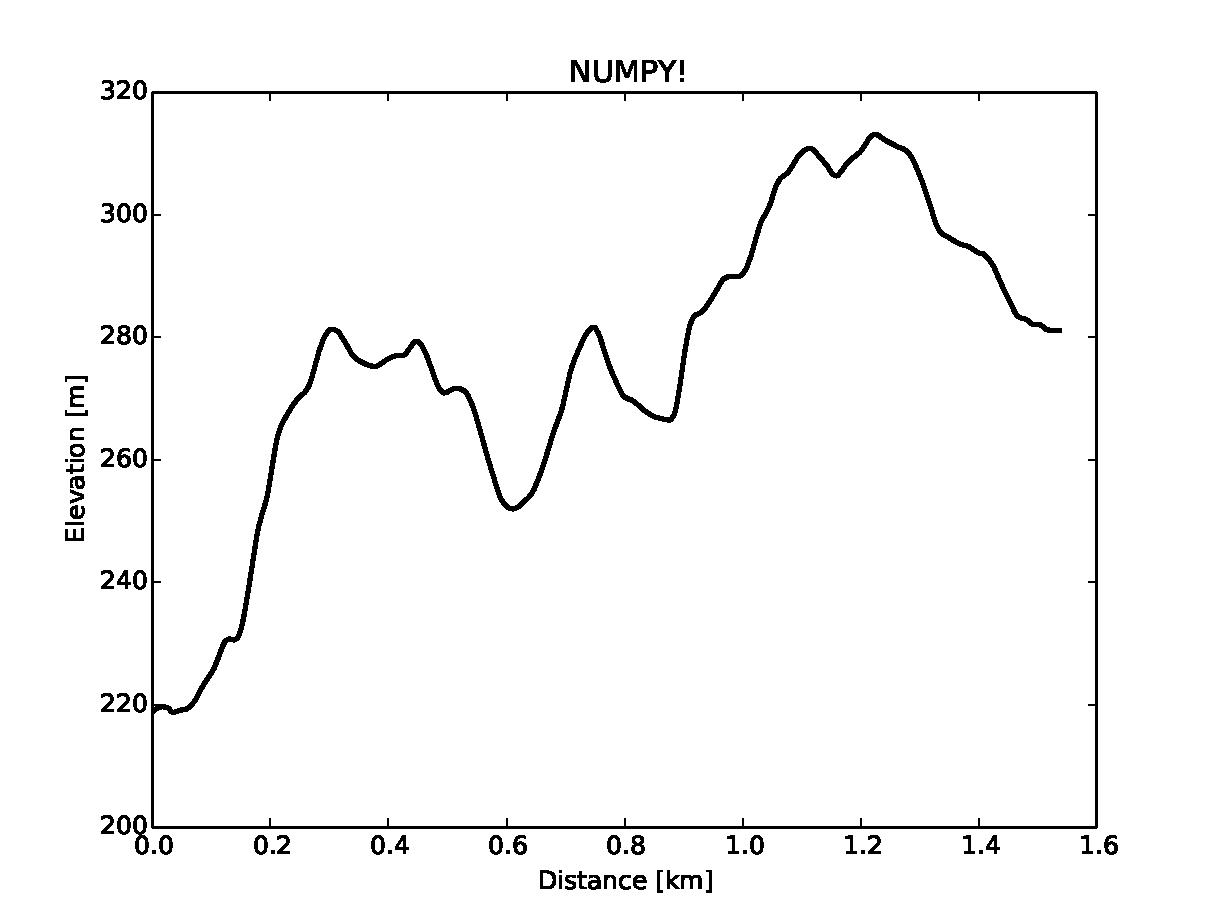
\includegraphics[width=.9\linewidth]{figures/FilesData/BattleCreekProfile.pdf}
\end{center}
\caption{Topographic profile from the Mississippi River valley (left) through tributary valleys and an end moraine complex (right).}
\end{figure}

\begin{framed}
\noindent\textbf{Time series and the datetime lilbrary}

If you want to work with time-series data, should look into the \lstinline{datetime} library for powerful functions to deal with date/time objects.
\end{framed}

You can also save ASCII data using the \lstinline{np.savetxt} feature. I mostly use it as follows:
\begin{lstlisting}
np.savetxt('OUTPUT_FILE_NAME.TXT', InputVariableName, fmt='%FORMAT_STRING')
\end{lstlisting}

Here, it is important to mention \textbf{formatting strings}. These follow the conventions from the C programming language. I will just introduce my most-used subset of them here.

Formatting strings contain a character. This determines how the incoming value is treated, but all output is as a string:
\begin{itemize}
 \item \lstinline{d}: integer
 \item \lstinline{f}: floating point (``float'')
 \item \lstinline{s}: string
\end{itemize}

These are then modified by numbers placed in front of the digits. Both the formatting string and the value that one would like to format as such must be preceded by a \lstinline{%}, and the formatting string must be inside quotes to denote that it is a string. I will explain through a set of examples:

\lstinputlisting{code/FilesData/formattingStrings.py}

\begin{framed}
\noindent\textbf{Saving multiple files with a numbering scheme}

In many cases, you may have data that belong in a particular order---whether they are a set of time-steps, a series of different analyses, or a number of different sample ID's that you want to automatically generate. For the case with real dates and times, you may use that date and time as part of the file name. And if you use it as \textbf{yyyymmdd}, it will alphabetically sort correctly! This becomes harder though if it is an arbitrary time step -- like say, millions of years ago, seconds, or just an arbitrary set of \textbf{[0, 1, 2, ..., 51, etc.]}. If you want the data to be sorted in order when you do a simple alphabetical sorting -- great for viewing in file browsers, loading into data analyses, or just for general orderly storage, you can run into the problem in which your data show up as \textbf{[0, 1, 10, 100, 2, ..., 51, etc.]}. This is certainly not what we want? So how do we fix it?

We use \textbf{zero-padding} (see code above on string formatting). So in our above example, if we can safely say that all the numbers are integers, and nothing will go over 9999, we can write an output file name as:

\lstinline{fnpadded = 'some_descriptive_text_' + '%04d' %time_step + '.ext'}

And then you can use this to save text output as a floating point with 2 decimal places of precision, called for example \lstinline{plate_reconstruction}, as follows:

\lstinline{np.savetxt(fnpadded, plate_reconstruction, fmt='%.2f')}

\end{framed}

Sometimes, ASCII data are not so easy to work with. This can happen when they are not in a simpe grid. In that case, we have to use lower-level Python commands. To learn basic file handling, you may see the help at \url{http://www.pythonforbeginners.com/files/reading-and-writing-files-in-python}.

One example of this sort of data is a set of GPS tracks provided by Ben P. These look something like:

\begin{lstlisting}
0
728609.215175176 7272865.670114477 3850.1122000000032
728608.813141581 7272866.856349733 3850.1769000000058
...
728588.585519101 7272909.968807690 3851.2842999999993
END
1
729772.085292112 7284330.246414313 3857.9808000000048
...
729789.783887492 7284223.112814812 3858.0691999999981
END
...
\end{lstlisting}

The numbers and ``END'' lines separate individual tracks. However, these are not nice 3-column entries. How do we parse a file like this?

Using the more basic Python file read/write commands (see links above), one can input the lines of the file, parse them into lists, and then turn them into arrays. This is as follows:

\lstinputlisting{code/FilesData/readGPStracks.py}

\begin{figure}[!ht]
\begin{center}
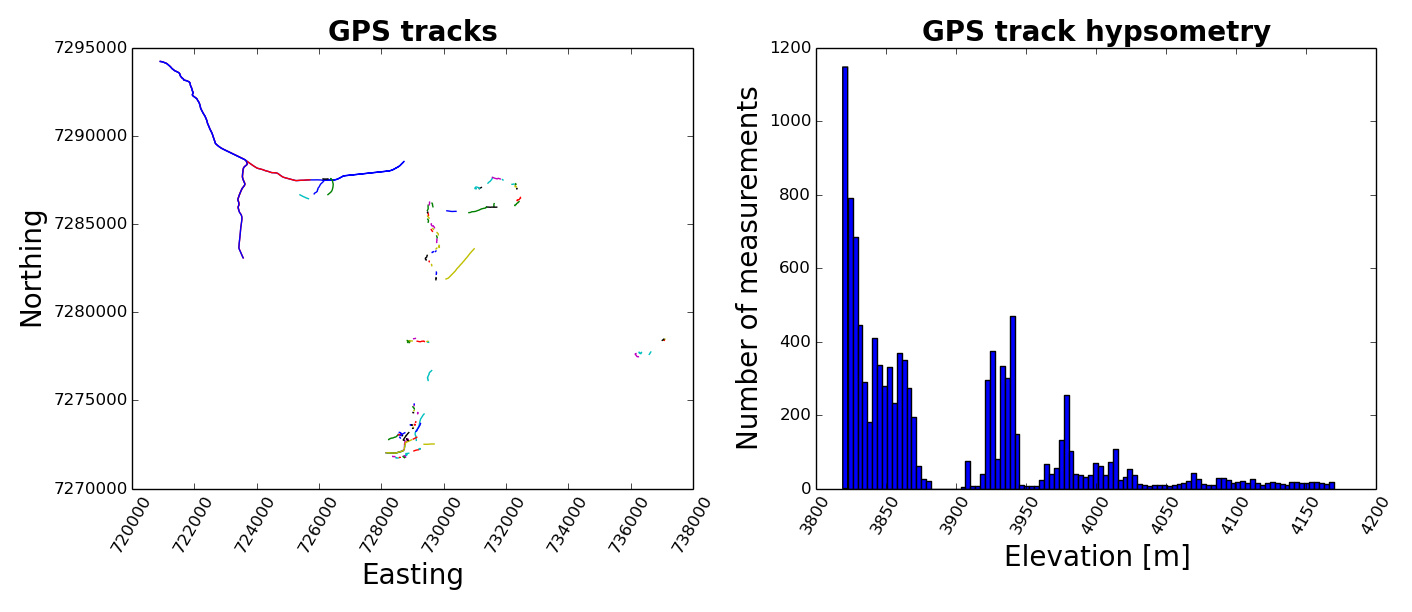
\includegraphics[width=.9\linewidth]{figures/FilesData/GPStracks.png}
\end{center}
\caption{GPS tracks (left) and hypsometry (right).}
\end{figure}

\section{Binary}

\subsection{Theory -- and how to get the most out of storage space}

Binary data are represented as a set of ones and zeros. In the Introductory notes, you learned how binary works, and a bit about how numbers may be generated.

Binary data are usually more compact than ASCII data, especially if used correctly. For example, a number between 0 and 65535 may be represented by two bytes (16 bits); this can be seen in binary because $2^16 = 65536$, and we want to include 0, so have to shift the maximum value down one. This is called a 16-bit unsigned integer, because it has 16 bits of data, and does not include a + or - sign (and hence is always positive). A number like this would require 5 bytes in ASCII to represent.

If you are representing a large number of binary values (0 or 1) as 16-bit unsigned integers, you would be using 2 bytes of data per value, while ASCII would require only 1 byte. So in this case, ASCII would be better! But this is where it becomes important to \textit{intelligentlly choose binary representations of data}. If we represented each of these values as binary logical values, each would only require 1 bit of storage space---an 8$\times$ improvement over ASCII and a 16$\times$ improvement over the 16-bit unsigned integer, which is really just too much storage space for binary data.

We often denote these values as follows:
\begin{itemize}
 \item unsigned integer: \lstinline{uint}
 \item signed integer (so can be $+$ or $-$): \lstinline{int}
 \item floating point: \lstinline{float}
\end{itemize}

You might also see terms like  \lstinline{single}, \lstinline{double}, \lstinline{char}, \lstinline{word}, etc.; these are less-descriptive terms that also relate to number of bytes in data. I use the three above to be more clear to those who have not memorized what all of these are.

These can also be used to denote how many bits are involved in each data type. For example:
\begin{itemize}
 \item unsigned 16-bit integer: \lstinline{uint16}
 \item signed 32-bit integer (so can be $+$ or $-$): \lstinline{int32}
 \item 64-bit floating point: \lstinline{float64}
\end{itemize}

\subsection{Practice -- raw binary files}

\lstinputlisting{code/FilesData/BinaryIO.py}

As a quick mental exercise, imagine that you have the numbers -15, 35, 119, and 43. What is the ideal number of bits with which to represent each number? How about 0, 50612, 151, 10512, 85, 3160? \textit{Answers: 8 bits (int8), 16 bits (uint16).}

\subsection{Binary containers}

\subsubsection{Numpy files}

Standard binary data formats are all right. But there are formats that can remember rows and columns of data, as well as ``container'' formats that can contain multiple arrays. So let's look at the native ones in numpy first.

\lstinputlisting{code/FilesData/npIO.py}

\subsubsection{Raster data -- a geospatial example}

Instead of just showing any standard raster data set, I am going to use a GeoTIFF that covers Berlin and the edge of Potsdam. In order to work with this, you are going to have to install the Python GDAL library.

\begin{framed}
\noindent\textbf{GDAL and OGR}
GDAL (raster) and OGR (vector) are the key software libraries behind most GIS applications. You can access them directly in Python, in additon to being able to access more general GIS libraries.
\end{framed}

Installing these libraries can be done with either your package manager (\lstinline{sudo apt-get install python-gdal}), or something like this), or with pip (\lstinline{sudo pip install gdal}). Seriously, do a good Google search about pip and how it works. It is super useful, with tools for remote sensing, dealing with mutliple data types, geological modeling, and of course lots of non-geological work.

\lstinputlisting{code/FilesData/GDAL_DEM.py}

\begin{figure}[!ht]
\begin{center}
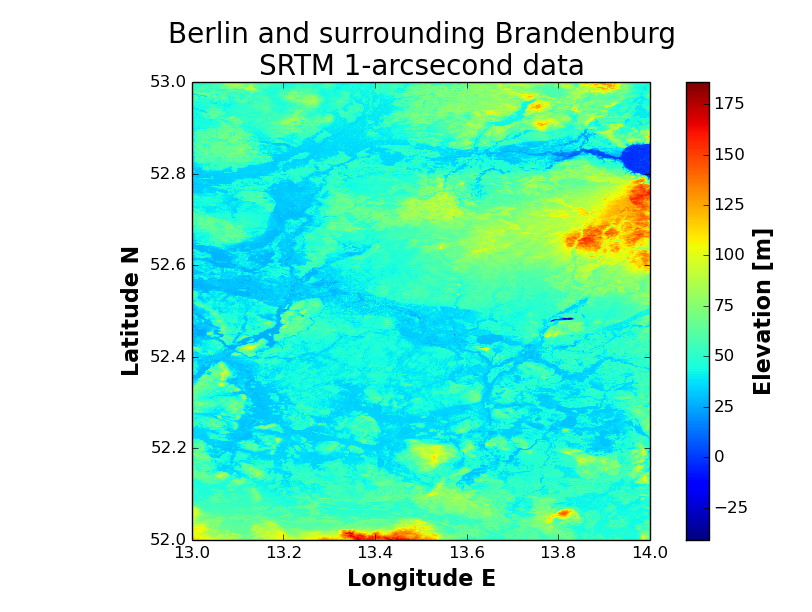
\includegraphics[width=.9\linewidth]{figures/FilesData/BerlinBrandenburgSRTM1as.png}
\end{center}
\caption{The DEM of the Berlin area does not show a ``well-ordered'' erosional fluvial landscape. Instead, it shows a landscape that has been greatly altered by glacial and fluvial processes around the ice margin.}
\end{figure}

\subsubsection{Working with NetCDF and HDF files -- in brief!}

These ``container'' file formats require special libraries to work with them. This is further complicated by the fact that there are different standards: NetCDF3 is being supplanted by NetCDF4, and HDF4 is still used for many satellite data sets but HDF5 being the better-supported current ``standard'' in Python. Did this last sentence just confuse you with too many acronyms? Me too! So let's try to simplify this problem.

First, install packages in the terminal (use ``sudo'' if you are on a UNIX-like system):
\begin{lstlisting}
pip install h4py
pip install netcdf4
\end{lstlisting}
In addition to these, there exists a NetCDF-3 library that is built-in to Scipy. Each of these has good help (and example) files. See:
\begin{itemize}
 \item h4py: \url{http://download.nexusformat.org/sphinx/examples/h5py/index.html} and \url{http://www.icare.univ-lille1.fr/howto_hdf/#data_extraction_Python}
 \item netCDF4 (works with NetCDF-4 and NetCDF-3 files): \url{https://github.com/erdc-cm/netCDF4-Python/blob/master/examples/tutorial.py}
 \item SciPy NetCDF: \url{http://docs.scipy.org/doc/scipy-0.14.0/reference/generated/scipy.io.netcdf.netcdf_file.html} (there used to be a more full tutorial but I cannot find it any longer)
\end{itemize}
In addition, this webpage has a lot of information on NetCDF (in general) and on the Basemap mapping toolkit, which will be discussed below: \url{http://www-pord.ucsd.edu/~cjiang/python.html}.

So it seems that in this case, the only thing that is left out is HDF4. What do we do with that? We convert it! Tools exist to convert HDF4 into either NetCDF or HDF5.
\begin{itemize}
 \item HDF4 $\rightarrow$ HDF5: \url{http://www.hdfgroup.org/h4toh5/} (main page); \url{http://www.hdfgroup.org/h4toh5/download.html} (Windows and Linux download); \url{http://hdfeos.org/software/h4toh5/bin/mac/} (Mac download)
 \item HDF4 $\rightarrow$ NetCDF4: \url{http://hdfeos.org/software/h4cflib.php}
\end{itemize}

Below, I have converted an HDF4 file from the TRMM satellite (Tropical Rainfall Measurement Mission) into a NetCDF-4 file, and import and plot it using Python. I first plot it using the standard matplotlib libraries, but later in the notes, use CartoPy to project it properly.

\lstinputlisting{code/FilesData/netCDF4basic.py}

\begin{figure}[!ht]
\begin{center}
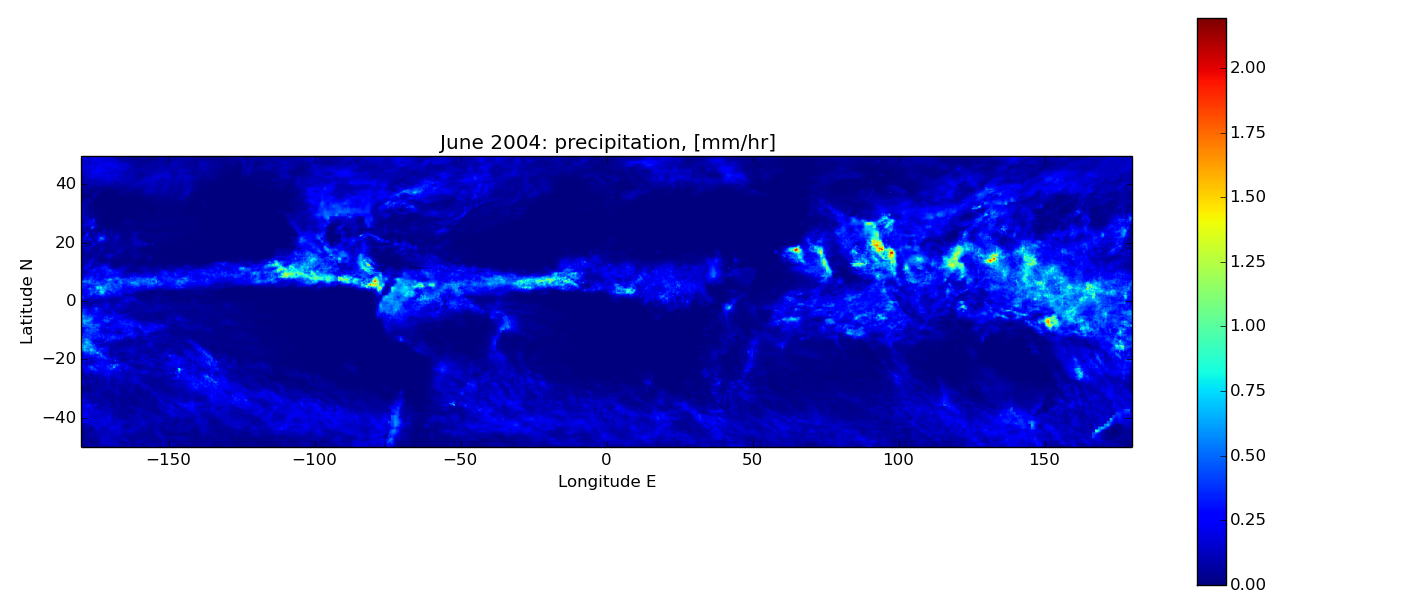
\includegraphics[width=.9\linewidth]{figures/FilesData/TRMM200406.png}
\end{center}
\caption{TRMM data from June 2004 (which is when the writer of these course notes graduated from high school).}
\end{figure}

\section{Working with Spreadsheets (Excel or LibreOffice Calc)}

So far, we've discussed all of these data formats that might be a bit more complex -- and these are all important for work with computers and larger data sets. However, many of us in the Earth sciences deal with spreadsheet data. Up until now, most (all?) of you have worked only by hand with this data. But no longer!

There many packages to work with spreadsheets. I will show you first the builtin method with Pandas here, but you should know about at least the two following ones (available via \lstinline{pip}):
\begin{itemize}
 \item openpyxl (Excel)
 \item odfpy (LibreOffice)
 \item oosheet (LibreOffice calc -- a spreadsheet-focused alternative to odfpy)
\end{itemize}

Here, we are going to plot an oxygen isotope history from a Greenland ice core:

\lstinputlisting{code/FilesData/GreenlandXLSXpandas.py}

\begin{figure}[!ht]
\begin{center}
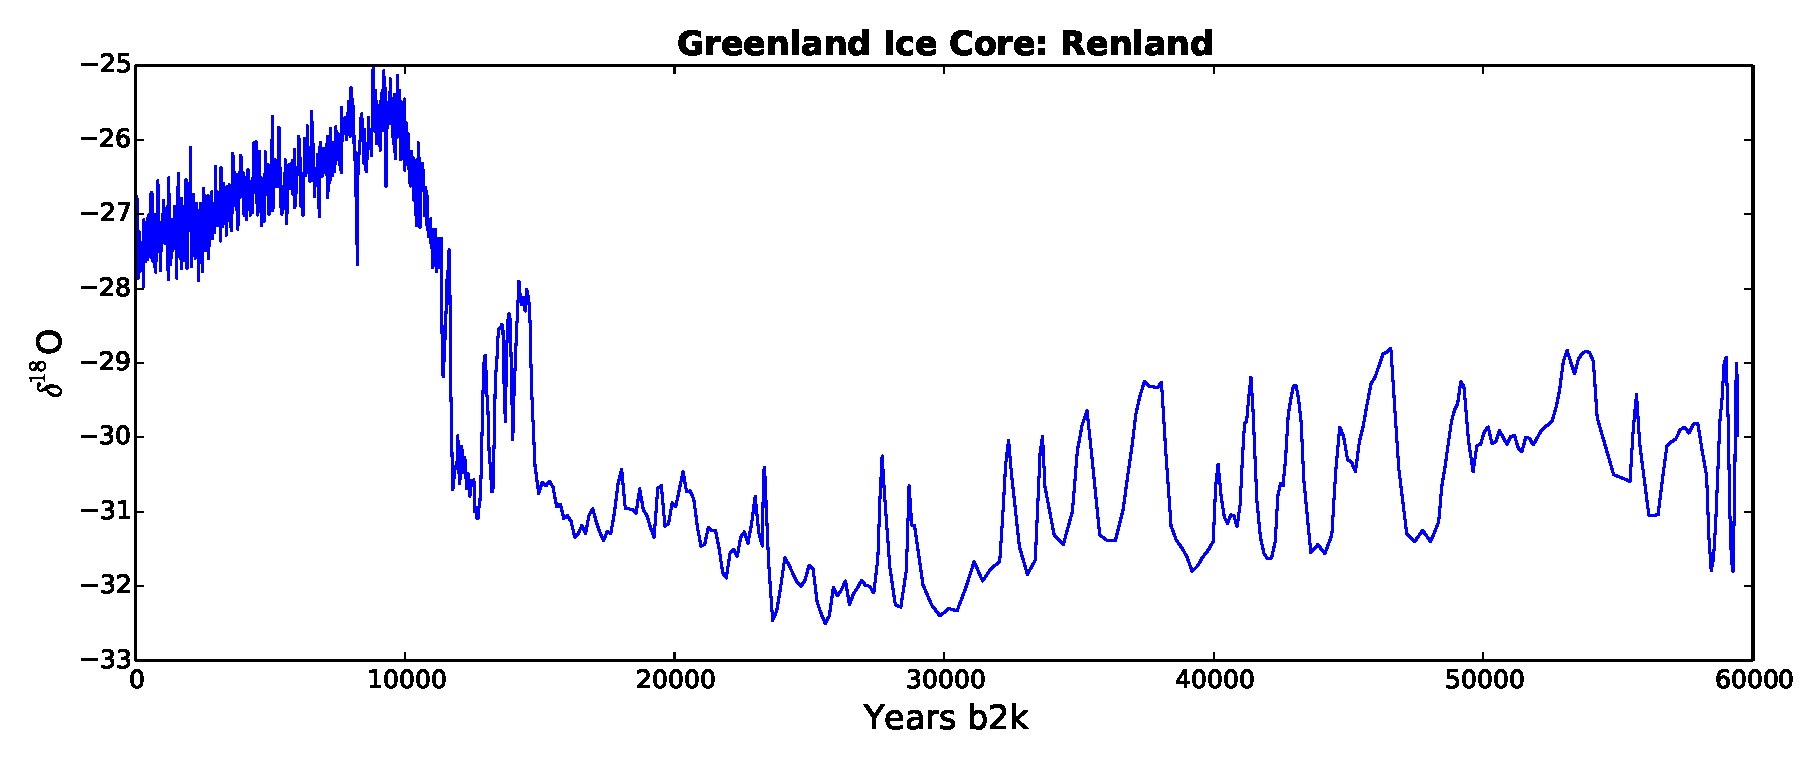
\includegraphics[width=.9\linewidth]{figures/FilesData/GreenlandRenlandXLS.pdf}
\end{center}
\caption{This is what the final graph of $\delta^{18}$O should look like from the above code. Up is warm and down is cold, roughly-speaking: these values are also related to global ice volume. Note the Bølling-Allerød warm period $\sim$14.5 ka, the Younger Dryas $\sim$11.7--13 ka, and the 8.2 ka event (the little negative spike in the Holocene related to catastrophic meltwater release from North American proglacial lakes into the North Atlantic ocean).}
\end{figure}

Openpyxl is also easy-to-use. Here is a quick example that I wrote for some real research -- to analyze sets of grain sizes of sediment from point counts of clasts. These data were transcribed from our field notebooks into a standard Excel format (thanks to Sara Savi), and I wrote the code that uses her standard Excel format to parse and compute statistics of different counts of grain size.

Go ahead and brainstorm how you might use this in your own work; we may spend some time going over this in class, as spreadsheets are really common.

\lstinputlisting{code/FilesData/GreenlandXLSXpandas.py}

\section{Stream gauging: an example}

\todo{Write new example for Monday with code from laptop that I wrote for the Mississippi}

\section{Plotting geospatial data using Basemap}

You might want to do some mapping without starting a full-fledged GIS. For that, I have often used the Python mapping toolkit called \lstinline{basemap}. This one cannot be installed via \lstinline{pip} or \lstinline{easy_install}: you will have to download it and run \lstinline{python setup.py install}. For instructions, see the Basemap toolkit webpage at \url{http://matplotlib.org/basemap/users/installing.html}. You can make really gorgeous maps with it; see \url{http://matplotlib.org/basemap/users/examples.html}.

There is also a newer mapping toolkit called CartoPy. It *is* available via pip, and you can read its help files at \url{http://scitools.org.uk/cartopy/docs/latest/index.html}. It is supposed to be better than Basemap in some ways (see \url{http://ocefpaf.github.io/python4oceanographers/blog/2013/09/23/cartopy/}), and has a really nice looking map gallery with good code examples provided as well \url{http://scitools.org.uk/cartopy/docs/latest/gallery.html} though as with many newer things, it is still in development.

\begin{framed}
\noindent\textbf{Additional help}

Additional support for numpy, matplotlib, and CartoPy can all be found in the SciTools GitHub repository at \url{https://github.com/SciTools/courses}.
\end{framed}

Here, I return to the TRMM dataset that we used earlier to show a global plot that is properly projected.

\lstinputlisting{code/FilesData/netCDFglobe.py}

\begin{figure}[!ht]
\begin{center}
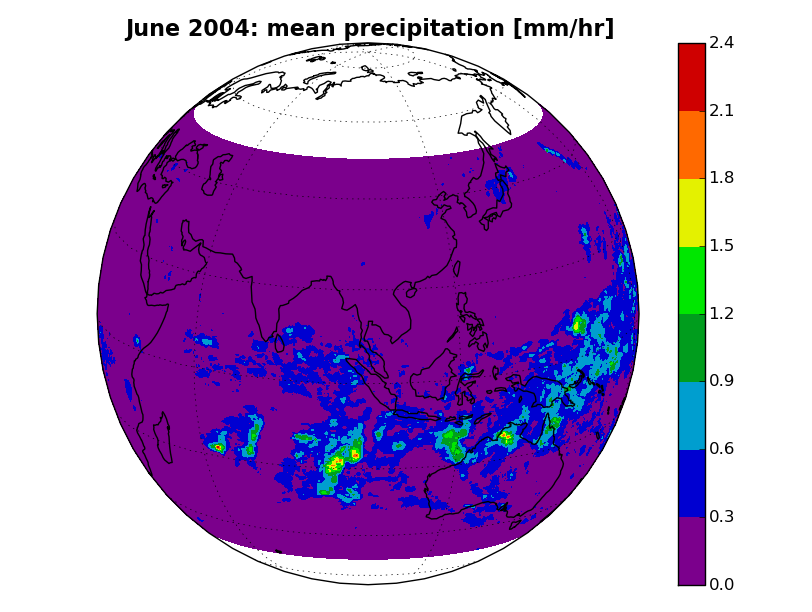
\includegraphics[width=.9\linewidth]{figures/FilesData/EasternHemispherePrecip.png}
\end{center}
\caption{TRMM data from June 2004 (which is when the writer of these course notes graduated from high school), now nicely plotted on a real Earth. Yes, we're getting closer to being computational Earth scientists!}
\end{figure}

\section{Plotting geospatial data using CartoPy}

\section{Python--GIS integration}

\subsection{GDAL and OGR}

\url{https://pcjericks.github.io/py-gdalogr-cookbook/}

\end{document}
